\documentclass{beamer}
%
% Choose how your presentation looks.
%
% For more themes, color themes and font themes, see:
% http://deic.uab.es/~iblanes/beamer_gallery/index_by_theme.html
%
\mode<presentation>
{
  \usetheme{Boadilla}      % or try Darmstadt, Madrid, Warsaw, ...
  \usecolortheme{beaver} % or try albatross, beaver, crane, ...
  \usefonttheme{default}  % or try serif, structurebold, ...
  \setbeamertemplate{navigation symbols}{}
  \setbeamertemplate{caption}[numbered]
  
} 

\usepackage{amsmath}
\usepackage{xcolor,colortbl}
\usepackage[english]{babel}
\usepackage[utf8x]{inputenc}
\usepackage{courier}
\usepackage{dsfont}
\usepackage{verbatim} 
\usepackage{enumerate}
\usepackage{tikz}
\usepackage{multirow}
\usepackage{venndiagram}
\usepackage{epigraph} 
%\usepackage{xcolor}
\newcommand{\xt}{\texttt}% \xt will be replaced with \textit
%\usepackage{enumitem}

\usepackage{hyperref}
\hypersetup{
    colorlinks=true,
    linkcolor=blue,
    filecolor=magenta,      
    urlcolor=cyan,
}

\usetikzlibrary{shapes,decorations,arrows,calc,arrows.meta,fit,positioning}
\tikzset{
    -Latex,auto,node distance =1 cm and 1 cm,semithick,
    state/.style ={ellipse, draw, minimum width = 0.7 cm},
    point/.style = {circle, draw, inner sep=0.04cm,fill,node contents={}},
    bidirected/.style={Latex-Latex,dashed},
    el/.style = {inner sep=2pt, align=left, sloped}
}

\setbeamertemplate{enumerate items}[default]
\graphicspath{{img/}}

%\setitemize{label=\usebeamerfont*{itemize item}%
%  \usebeamercolor[fg]{itemize item}
%  \usebeamertemplate{itemize item}}

\newcommand{\Mypm}{\mathbin{\tikz [x=1.4ex,y=1.4ex,line width=.1ex] \draw (0.0,0) -- (1.0,0) (0.5,0.08) -- (0.5,0.92) (0.0,0.5) -- (1.0,0.5);}}%




\title[SST-115 / STA-209]{Numerical Summaries}
\subtitle{}
\author{Grinnell College}
\date{September 16, 2024}

\begin{document}

\begin{frame}
  \titlepage
\end{frame}


\begin{frame}{Review}
Graphical Summaries:
\begin{itemize}
\item Why do we create graphs?
\item Types of plots
\item Describing plots
\end{itemize}
\vspace{4mm}

We will now spend some more time on describing quantitative variables
\end{frame}



\begin{frame}{Review -- One Quantitative Variable}
We've seen a few examples of histograms at this point.
\begin{columns}
  \begin{column}{0.45\textwidth}
	\begin{center}
	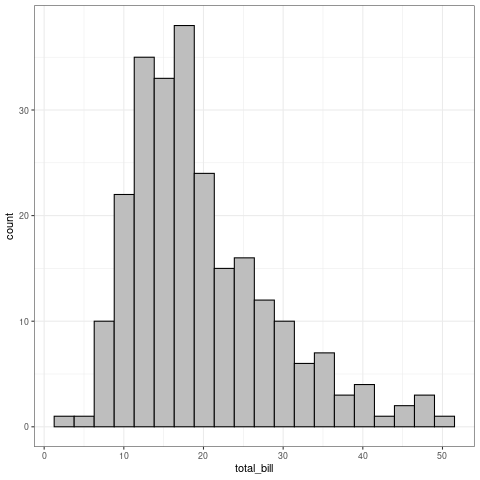
\includegraphics[scale=0.35]{img/bill_bin_20.png}
	\end{center}
  \end{column}
  \begin{column}{0.45\textwidth}
	Some of the things we've thought about:
	\begin{itemize}
	\item What are the most common values?
	\item How spread out is this data?
	\item What about the range of this data?
	\item Does it appear skewed or symmetric?
	\end{itemize}
  \end{column}

\end{columns}
\end{frame}



\begin{frame}{Review}
We spent some class time over the last 2 weeks learning how to talk about our data. Largely our time has been spent on both of these:\vspace{4mm}

\begin{enumerate}
    \item \textbf{Data Visualization} displaying data in ways that make patterns more noticeable
    \item \textbf{Numerical Summaries} calculating numbers that tell us about certain aspects of the data
\end{enumerate}\vspace{4mm}

Often these concepts ended up getting combined in that we would use numerical summaries to help us describe our graphs and plots. We are going to spend a bit more time today learning about numerical summaries.
\end{frame}



\begin{frame}{Review -- Quantitative Distribution}
We need to mention all of the following things when we describe the \textbf{distribution} of a quantitative variable:\vspace{3mm}

\begin{itemize}%[leftmargin=1em]
 \item \textbf{Shape} - how does the distribution look?
    \begin{itemize}
        \item - symmetric?
        \item - skewed?
        \item - $\#$ of modes
    \end{itemize}
 \item \textbf{Center} - where does the data bunch up
 \item \textbf{Spread} - how spread out is the data
 \item \textbf{Outliers} - are there values that are much smaller/larger than the rest?
\end{itemize}
\end{frame}



\begin{frame}{Numerical Summaries}
The \textbf{center} of a quantitative variable is meant to help us answer
\begin{itemize}
    \item What are the most common values?
    \item Where does the data bunch up?
    \item What is the 'typical' value that most observations had?
\end{itemize} \vspace{4mm}


The \textbf{spread} of a distribution is meant to tell us, literally, how spread out the values are. \textbf{Spread} also tells us how much \textit{variability} there is \vspace{5mm}

There are two separate approaches for describing center and spread \\ \vspace{2mm}

\begin{enumerate}
\item Order Statistics
\item Moment Statistics
\end{enumerate}
\end{frame}



\begin{frame}{Order Statistics}
\textbf{Order statistics} are numerical summaries based on the ordered ranking of a quantitative variable (smallest to largest) \vspace{4mm}

There are a few properties in particular that make order statistics useful:
\begin{enumerate}
\item They make no assumptions about how the data is distributed
\item Are generally robust to (unaffected by) major fluctuations in the data (i.e., outliers)
\item Easier to interpret
\end{enumerate} \vspace{4mm}
\end{frame}



\begin{frame}{Review -- Percentiles}
A \textbf{percentile} $\alpha$ is a number such that $\alpha\%$ of our (quantitative) observations fall at or below this number when ranked from smallest to largest \vspace{5mm}

Some percentiles have special names. The \textit{median}, for example, is the 50th percentile. \vspace{5mm}

Other notable percentiles include:
\begin{enumerate}
\item Minimum
\item 25th percentile or \textbf{first quartile} ($Q_1$)
\item 75th percentile or \textbf{third quartile} ($Q_3$)
\item Maximum
\end{enumerate}
\vspace{3mm}
\end{frame}



\begin{frame}{Median (Center)}
The \textbf{median} is another name for the 50th percentile. It is frequently used as a measure of center.\vspace{6mm}

These are some other ways to think about the \textbf{median}.
\begin{itemize}
    \item the \textbf{median} divides the data into an upper and lower half
    \item  the middle value of the data if arranged from smallest to largest
    \item about half the data is larger than the median and about half the data is smaller
\end{itemize}
\end{frame}



\begin{frame}{IQR (Spread)}
The IQR is a measure of the spread of our data.
\begin{itemize}
    \item calculation is Q3 - Q1
    \item measures the range of the middle 50$\%$ of the data
\end{itemize}
\begin{center}
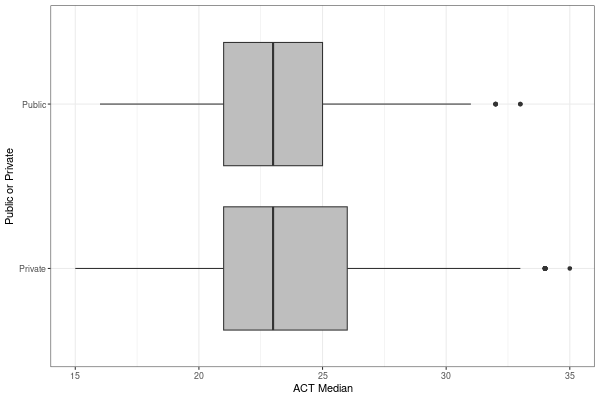
\includegraphics[scale=.35]{img/box_private.png}
\end{center}
\end{frame}



\begin{frame}{Five Number Summary}
\begin{center}
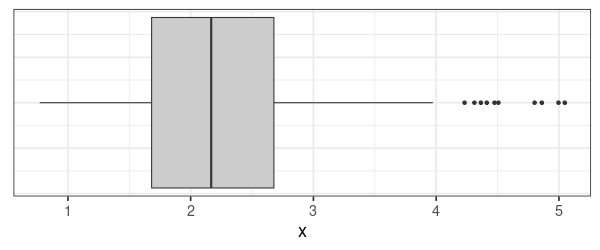
\includegraphics[scale=0.5]{box.png}
\end{center}
\begin{columns}

  \begin{column}{0.45\textwidth}
\begin{itemize}
\item Median
\item 25th Percentile ($Q_1$)
\item 75th Percentile ($Q_3$)
\end{itemize}
  \end{column}
  \begin{column}{0.45\textwidth}
\begin{itemize}
\item Minimum or 1.5 $\times$ IQR
\item Maximum or 1.5 $\times$ IQR
\item Outliers
\end{itemize}
  \end{column}
\end{columns}
\end{frame}



\begin{frame}{Moment Statistics}
\textbf{Moment statistics} are statistics that are based on specific mathematical properties of our data. There are some very powerful math tools that can make use of these (we will see some shortly) \vspace{12mm}

Unlike order statistics, moment statistics (largely) \textit{do} make assumptions about how the data is distributed: as such, they can be very sensitive to unexpected fluctuations such as outliers \vspace{4mm}

In this sense, we say that moment statistics \textit{are not} robust
\end{frame}



\begin{frame}{Some Notation}
Before we continue, it is helpful to introduce some notation that can make doing calculations with data a little easier. \vspace{4mm}

\textbf{n} is often used to denote the sample size ($\#$ of observations in our sample) \vspace{4mm}

\textbf{x$_i$} is used to denote the values for a variable in our data set

i.e.: \textbf{x}$_3$ is the 3rd value of the variable in the data set \vspace{4mm}

$\sum$ is a symbol frequently used to denote adding a whole bunch of things together.
\end{frame}



\begin{frame}{Mean (Center)}
The \textbf{mean} is the same thing as the \textbf{average} value of the variable.\vspace{4mm}

To find the value of the mean, we add up all the values of the variable and divide by the number of observations.\vspace{4mm}

Often the \textit{sample} \textbf{mean} of a variable is denoted as \textbf{$\overline{x}$}\vspace{4mm}

Using the notation from the previous slide, the equation for the \textbf{mean} is
\begin{equation*}
\overline{x} = \frac{\sum x_i}{n}
\end{equation*}
\end{frame}



\begin{frame}{Spread -- Standard Deviation}
\textbf{Standard Deviation} -- a way of measuring the typical deviation (distance) of each observation from the \textit{mean}
\begin{itemize}
    \item the symbol \textbf{s} is often used to denote the standard deviation of our sample (sample standard deviation)
\end{itemize}
\begin{align*}
s = \sqrt{\frac{1}{n-1} (x_i - \overline{x})^2 }
\end{align*}

\textbf{Why do we take the square root?}
Taking the square root ensures that the standard deviation has the same units as the original variable\vspace{4mm}

\textbf{Why do we use n-1 and not n?}
It's complicated. Using n-1 gives us better estimates and predictions
\end{frame}



\begin{frame}{Standard Deviation}
Some properties of the \textbf{standard deviation}:
\begin{itemize}
    \item measures spread (variability) from the mean
    \begin{itemize}
        \item values close to the mean = smaller contribution to s
        \item values far away from the mean = larger contribution to s
    \end{itemize}
    \item cannot be negative (s $\geq 0$)
    \item has the same units as the original variable
\end{itemize}\vspace{8mm}

You may hear the word \textbf{variance}.
\begin{itemize}
    \item variance = $s^2$
    \item harder to interpret
    \item certain math scenarios where it is easier to work with than s
\end{itemize}
\end{frame}



\begin{frame}{Which measures to use?}
The \textit{shape} of the distribution, as well as whether we have \textit{outliers} will determine whether we use \textbf{order statistics} (median and IQR) or \textbf{moment statistics} (mean and standard deviation) to describe the center and spread \vspace{6mm}

In general we prefer to use \textbf{moment statistics} (mean and standard deviation) if we can, but there are certain situations where the mean and standard deviation are not good measures of center and spread
\end{frame}

\begin{frame}{Which measures to use?}
Order statistics are robust, moment statistics are not robust.
\begin{itemize}
    \item A skewed distribution can affect the mean and std. dev. a lot
    \begin{itemize}
        \item skew $\rightarrow$ mean $\&$ std. dev. not good measures of center $\&$ spread
    \end{itemize} \vspace{2mm}
    \item Outliers can affect the mean and std. dev. a lot
    \begin{itemize}
        \item outliers $\rightarrow$ mean $\&$ std. dev. not good measures of center $\&$ spread
    \end{itemize}
\end{itemize} \vspace{4mm}

Summary:
\noindent\fbox{\begin{minipage}{.9\textwidth}
Symmetric shape with no 'extreme' outliers $\rightarrow$ mean and std. dev.

Skewed shape or outliers (or both) $\rightarrow$ median and IQR
\end{minipage}}
\end{frame}



\begin{frame}{Comparing Mean with Median}
\begin{center}
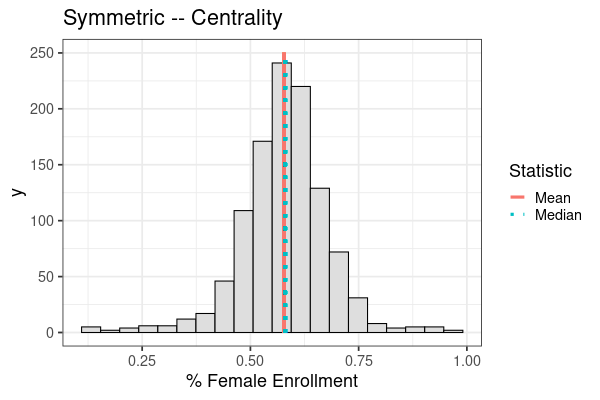
\includegraphics[scale=0.5]{center_sym.png}
\end{center}
\end{frame}



\begin{frame}{Comparing Mean with Median}
\begin{center}
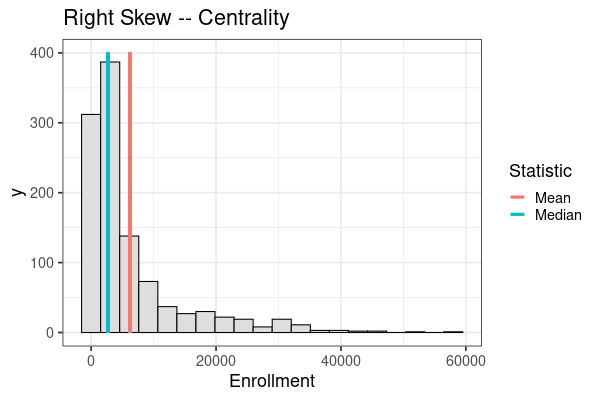
\includegraphics[scale=0.5]{center_skew.png}
\end{center}
\end{frame}




\begin{frame}{Practice}

{\small
For each of the following variables visualized below:
\begin{enumerate}
\item Determine approximate mean and median and which should be larger. How do you know?
\item Decide whether standard deviation or IQR is more appropriate for describing variability
\end{enumerate}
}
\begin{center}
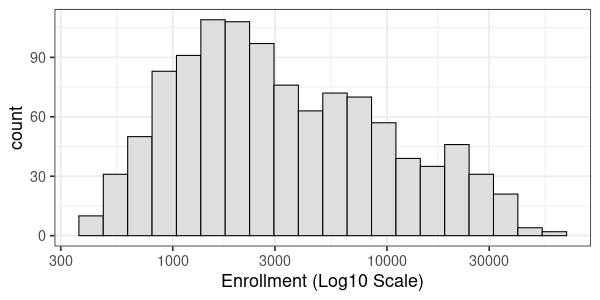
\includegraphics[scale=0.5]{mult_dist3.png}
\end{center}
\end{frame}



\begin{frame}{Practice}

{\small
For each of the following variables visualized below:
\begin{enumerate}
\item Determine approximate mean and median. Are they very different?
\item Decide whether standard deviation or IQR is more appropriate for describing variability
\end{enumerate}
}
\begin{center}
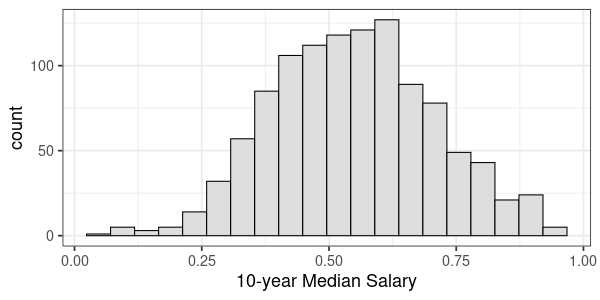
\includegraphics[scale=0.5]{mult_dist2.png}
\end{center}
\end{frame}



\begin{frame}{Practice}
Describe the distribution of '$\%$ White Enrollment.'
\begin{center}
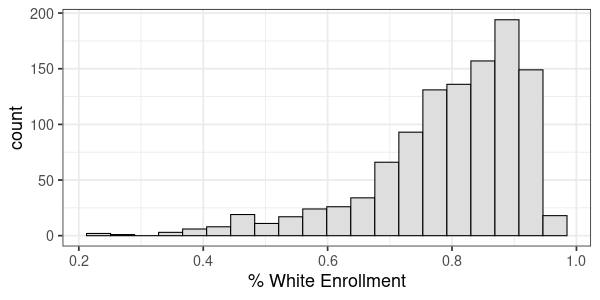
\includegraphics[scale=0.5]{mult_dist1.png}
\end{center}
\end{frame}



\begin{frame}{Practice}
Describe the distribution of Median Debt. 
\begin{center}
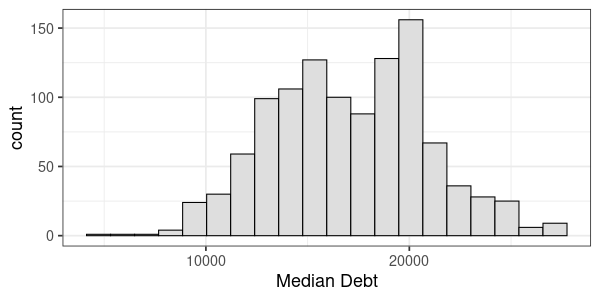
\includegraphics[scale=0.5]{mult_dist4.png}
\end{center}
\end{frame}



\begin{frame}{Advantages and Disadvantages}
\begin{columns}

  \begin{column}{0.45\textwidth}
\textbf{Order Statistics} \\ \vspace{2mm}
Advantages:
\begin{itemize}
\item[] Robust to outliers 
\item[] More ``correct" center for skew
\end{itemize}
Disadvantages:
\begin{itemize}
\item[] Discards most data
\item[] No nice math properties
\end{itemize}
  \end{column}
  \begin{column}{0.45\textwidth}
\textbf{Moment Statistics} \\ \vspace{2mm} 
Advantages:
\begin{itemize}
\item[] Very useful math properties 
\item[] Utilizes all of the data
\end{itemize}
Disadvantages:
\begin{itemize}
\item[] Sensitive to outliers
\item[] Sensitive to skew
\end{itemize}
  \end{column}

\end{columns}
\end{frame}


\begin{frame}{Comparing Quantitative Variables}
We can use \textbf{center} and \textbf{spread} to compare distributions. We typically refer to measures of centrality when discussing association. \vspace{3mm}


Consider the five-number summary for our Enrollment variable ($\#$ students enrolled at a college)
\begin{table}[ht]
\centering
\begin{tabular}{rrrrrrr}
  \hline
 & Min. & 1st Qu. & Median & Mean & 3rd Qu. & Max. \\ 
  \hline
 & 401 & 1388 & 2733 & 6241 & 7272 & 58392 \\ 
   \hline
\end{tabular}
\end{table}
\vspace{3mm}

Now lets look at the same variable, but add in info Public/Private
% latex table generated in R 4.3.2 by xtable 1.8-4 package
% Thu Feb  8 12:40:51 2024
\begin{table}[ht]
\centering
\begin{tabular}{rrrrrrr}
  \hline
 & Min. & 1st Qu. & Median & Mean & 3rd Qu. & Max. \\ 
  \hline
Private & 405 & 1079 & 1725 & 2720 & 2938 & 45370 \\ 
  Public & 401 & 3788 & 7803 & 11325 & 17152 & 58392 \\ 
   \hline
\end{tabular}
\end{table}
\end{frame}



\begin{frame}{Conditional Statistics}
Which type of college tends to have more students enrolled? (center)
\begin{center}
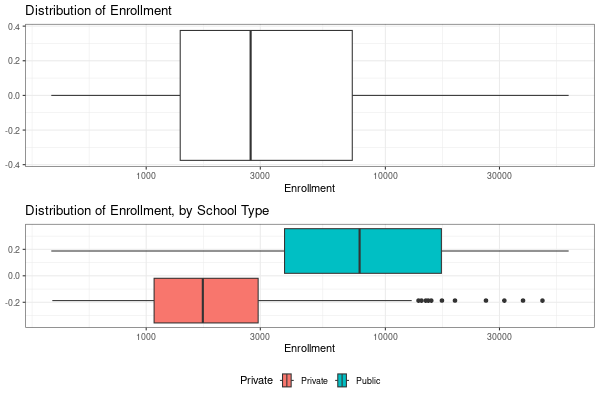
\includegraphics[scale=0.5]{enrollment_conditional.png}
\end{center}
\end{frame}



\begin{frame}{Parameter vs Statistics}
Sometimes we will need to distinguish whether we are talking about things like mean/median/IQR/Std. dev. for a sample of data or for a population\vspace{4mm}

\textbf{Statistics} are numerical summaries calculated from the \textit{sample}.
\begin{itemize}
    \item typically statistics are denoted using lowercase English alphabet characters
        \begin{itemize}
            \item sample mean = $\overline{x}$
            \item sample standard deviation = s
        \end{itemize}
\end{itemize} \vspace{3mm}

\textbf{Parameters} are numerical summaries calculated from the population.
\begin{itemize}
    \item typically parameters are denoted using Greek alphabet characters
        \begin{itemize}
            \item population mean = $\mu$
            \item population standard deviation = $\sigma$
        \end{itemize}
    \item almost always the value of parameters are unknown to us (we want to learn about their values)
\end{itemize}
\end{frame}



\begin{frame}{Z-scores}
Sometimes we want to compare two variables that measure similar things but use different scales. (i.e.: ACT or SAT exam scores) \vspace{3mm}

\textbf{Standardizing} our values is a way of adjusting them so that we can directly compare them. These adjusted values are called \textbf{z-scores}. \vspace{10mm}

There are two formulas for calculating z-scores depending on if we are using sample or population info
\begin{columns}
  \begin{column}{0.45\textwidth}
        \begin{align*}
            z_i = \frac{x_i - \overline{x}}{s_x}
        \end{align*}
  \end{column}
  \begin{column}{0.45\textwidth}
        \begin{align*}
            z_i = \frac{x_i - \mu}{\sigma}
        \end{align*}
  \end{column}
\end{columns} \vspace{2mm}
\begin{itemize}
    \item in order to use $\mu$ and $\sigma$ you need to actually be told these values, often a question prompt will tell you what to use
\end{itemize}
\end{frame}



\begin{frame}{Z-score Properties}
We can talk about standardizing a single value or an entire variable (standardizing \textit{all} values of the variable) \vspace{3mm}

If we standardize a variable, what we are doing is scaling each value so that the mean becomes 0 and the standard deviation becomes 1. \vspace{3mm}

Properties of Z-Scores
\begin{itemize}
    \item puts values on the same scale
    \item mean (center) = 0, std. dev (spread) = 1
    \item no units
    \item does not change the overall shape of the distribution
\end{itemize}
\end{frame}



\begin{frame}{Z-Score Comparisons}
Z-score interpretation:
The value we get is the number of standard deviations the value is away from the mean
\begin{itemize}
    \item positive z-scores are larger than the mean
    \item negative z-scores are smaller than the mean
\end{itemize} \vspace{4mm}

Examples 
\begin{itemize}
    \item If z = 1.5, then the observation is 1.5 standard deviations larger than the mean
    \item If z = -1, then the observation is 1 standard deviation less than the mean
\end{itemize}
\end{frame}

\begin{frame}{Example (Grinnell)}
In our college dataset: 
\begin{itemize}
    \item the average ACT Median is $\overline{x} = 23.58$
    \item standard deviation of $s_x = 3.55$
\end{itemize} \vspace{6mm}

Grinnell College has a median ACT of 32
\begin{itemize}
\item We can calculate its standardized value as:
\begin{align*}
z_{Grinnell} = \frac{32 - 23.58}{3.55} = 2.37
\end{align*}
\item This indicates that the median ACT at Grinnell College is 2.37 standard deviations above the average
\end{itemize}
\end{frame}



\begin{frame}{Example (Iowa State University)}
In our college dataset: 
\begin{itemize}
    \item the average ACT Median is $\overline{x} = 23.58$
    \item standard deviation of $s_x = 3.55$
\end{itemize} \vspace{6mm}

Iowa State University has a median ACT of 25
\begin{itemize}
\item We can calculate its standardized value as:
\begin{align*}
z_{ISU} = \frac{25 - 23.58}{3.55} = 0.40
\end{align*}
\item This indicates that the median ACT at ISU is 0.4 standard deviations above the average
\end{itemize}
\end{frame}



\begin{frame}{Example (Comparison)}
We can compare Grinnell to ISU in terms of either mean 'ACT Median' directly, or we can compare their z-scores.

\begin{center}
\begin{align*}
ACT_{Grinnell} = 32, \hspace{8mm} ACT_{ISU} = 25\\
z_{Grinnell} = 2.37, \hspace{10mm} z_{ISU} = 0.40
\end{align*} 
\end{center}
Which has the better score? 

Grinnell, since the z-score is larger
\end{frame}



\begin{frame}{Another example (ACT vs SAT)}

\noindent\fbox{\begin{minipage}{.9\textwidth}
\begin{itemize}
    \item \small The average score on the ACT English exam is 21.0 with a standard deviation of 4.0.
    \item \small The average score on the SAT Verbal exam is 520 with a standard deviation of 100.
    \item \small Kala scored a 27 on the ACT English exam.
    \item \small Nia scored a 770 on the SAT Verbal exam.
\end{itemize}
\end{minipage}} \vspace{4mm}

\begin{equation*}
    z_{Kala}=\frac{27-21}{4} = 1.5 \hspace{10mm} z_{Nia} = \frac{770-520}{100} = 2.5
\end{equation*} \vspace{4mm}

\textbf{Who scored better?} Nia, since Nia's z-score is larger
\end{frame}


\begin{frame}{Transformation}
\footnotesize
We can \textbf{standardize} all the values of a variable. The resulting standardized Values are either squeezed or stretched, but their relative positions stay the same

\begin{center}
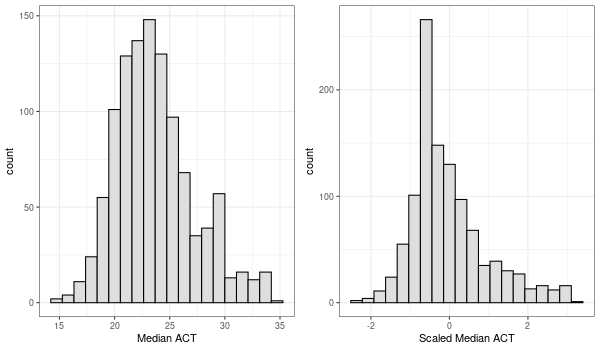
\includegraphics[scale=0.5]{scaled_act.png}
\end{center}
\end{frame}

\begin{frame}{Transformation}
\footnotesize
Similar to IQR giving us a range of common values, sometimes mean and standard deviation are used to create ranges of common values. Nearly the same amount of data still falls within this interval \vspace{3mm}

Mean and one standard deviation:
\begin{center}
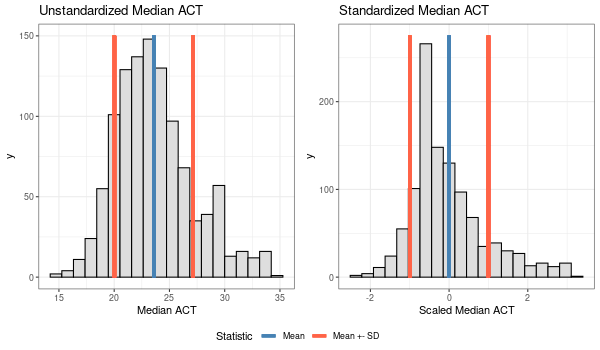
\includegraphics[scale=0.5]{scaled_act2.png}
\end{center}
\end{frame}

\begin{frame}{Transformation}
\footnotesize
Mean and two standard deviations
\begin{center}
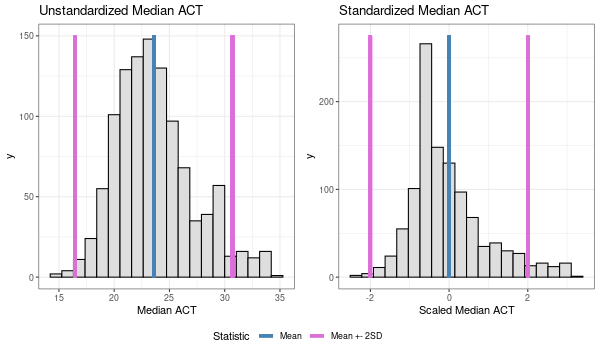
\includegraphics[scale=0.5]{scaled_act3.png}
\end{center}
\end{frame}



\begin{frame}{68-95-99 Rule}
Useful property of the mean and standard deviation when we have a bell-shaped distribution (unimodal and symmetric).
\begin{center}
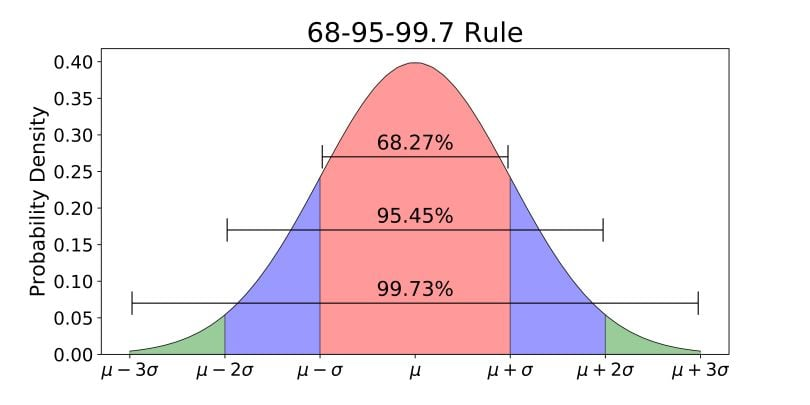
\includegraphics[scale=0.4]{empirical_rule.jpg}
\end{center}
\end{frame}


%%%%%%%%%%%%%%%%
\begin{frame}{Review}

\begin{enumerate}
\item What is the difference between Order and Moment statistics?
\item What are the measures of center and spread we saw?
\item How do shape/outliers affect the measures of center/spread we use?
\item What is the purpose of standardizing a variable?
\end{enumerate} \vspace{10mm}

Additional question: Do you prefer examples where I write answers on the board, or do you prefer me putting them in the slides and explaining the answer (board / slides)
\end{frame}


\end{document}
